\chapter{电路基础}\label{dianlujichu}

\begin{introduction}
\item \nameref{sec10}
\item 基础电路示例
\item 逻辑门基础
\end{introduction}

\section{电源/电线/用电器}\label{sec10}

在现实生活中,电路的三个基本组成部分为电源、导电回路和用电器,电源产生的电流经回路传导到用电器并驱动用电器。在泰拉瑞亚中,电路的三个基本组成部分为电源、电线和用电器,电源产生的电信号经电线传导到用电器,用电器响应该电信号。wiki上这样描述这个过程:电源激活——电源上的电线激活——电线下的用电器激活。在本书接下来的讨论中,我们采用wiki上的解释,统一使用激活(activate)来表达电路的活跃状态。

由于电线和图格处于不同图层,它们可以重叠。如果某电线与某图格重叠,我们说该图格在该电线下,该电线在该图格上。

电源指可激活其上电线的图格或该图格对应的物品,每个电源有其特有的激活条件。用电器指可被其上电线激活的图格或该图格对应的物品,每个用电器被激活时有其特有的响应方式。泰拉瑞亚中所有电源及其激活条件见\autoref{dianyuan},所有用电器及其响应方式见\autoref{yongdianqi},详细信息请参阅\nameref{sec1}及wiki。

\begin{longtable}{|c|c|}
\caption{泰拉瑞亚中的电源}\label{dianyuan}\\\hline
电源					&	激活条件					\\
\hline
\endfirsthead
\hline
电源					&	激活条件					\\
\hline
\endhead
\hline
\endfoot
开关/控制杆				&	鼠标右击					\\
\hline
灰/棕/蓝/丛林蜥蜴压力板	&	玩家踩踏					\\
\hline
红/绿压力板				&	玩家/NPC/敌怪踩踏			\\
\hline
黄压力板				&	NPC/敌怪踩踏				\\
\hline
加重压力板				&	玩家踩上或离开				\\
\hline
青绿压力垫板			&	射弹触碰					\\
\hline
1/3/5秒计时器			&	开启后每隔1/3/5秒激活		\\
\hline
引爆器					&	玩家自上而下冲击或鼠标右击	\\
\hline
宝石锁					&	对应的大宝石被嵌入或取出	\\
\hline
受困宝箱				&	鼠标右击					\\
\hline
逻辑感应器(昼/夜)		&	入昼/入夜					\\
\hline
逻辑感应器(玩家)		&	玩家进或出蓝色方框			\\
\hline
液体感应器				&	对应液体进入或离开			\\
\hline
逻辑门					&	详见后文					\\
\end{longtable}

\begin{longtable}{|c|c|}
\caption{泰拉瑞亚中的用电器}\label{yongdianqi}\\\hline
用电器		&	响应方式	\\\hline
\endfirsthead
\hline
用电器		&	响应方式	\\\hline
\endhead
\hline
\endfoot
部分光源	&	亮/灭切换	\\\hline
门、机关门、高门&	开/关切换	\\\hline
泵	&把入水泵上的液体传送到出水泵	\\\hline
机关	&	发射射弹/爆炸并消失	\\\hline
炮台&根据激活点改变方向/射击\\\hline
烟花喷泉、烟花盒&产生烟花\\\hline
烟花火箭&发射\\\hline
泡泡机、呆萌气球机、派对中心&开/关切换,生成背景特效\\\hline
喷泉&开/关切换,改变水的颜色\\\hline
八音盒&开/关切换,改变背景音乐\\\hline
部分雕像&\makecell{生成物品/传送城镇NPC/亮灭切换/\\生成敌怪/生成小动物}\\\hline
烟囱&三个状态切换\\\hline
传送机&交换两个传送机上的玩家和NPC\\\hline
天塔柱&开/关切换,改变背景\\\hline
广播盒&显示文字讯息\\\hline
传送带&改变方向\\\hline
制动器&切换图格的虚化状态\\\hline
彩线灯泡&四色电线各控制一个灯泡的亮灭\\\hline
像素盒&\makecell{从左/右激活时熄灭,\\同时从上/下和左/右激活时点亮}\\\hline
逻辑灯&详见后文\\\hline
矿车轨道交叉点&在两种交叉方式中切换
\end{longtable}

最简单的电路包含一个电源、一个用电器,以及连接电源与用电器的电线。在这个电路中,激活电源的瞬间,用电器会被自动激活。读者可以尝试用电线连接各种各样的电源和用电器,然后尝试激活电源,看看会发生什么。

\begin{example}
用火把摆出数字“0”(\autoref{i32}),然后用电线连接一个开关和“0”左边三条边(\autoref{i33})。在这个电路中,开关是电源,“0”的左边三条边上的火把是用电器。因为开关的激活条件是右击,我们右击开关就能激活它,然后开关上的红线激活,于是红线下“0”的左边三条边被激活。火把的激活响应是亮灭切换,所以这三条边就会灭,显示数字“1”(\autoref{fig74})。反复右击开关,这些火把就会在亮灭之间切换,从而显示的数字在“0”和“1”之间切换。这就是最简单的二进制\textbf{数显},数显是数字显示器的简称。

\begin{figure}[!ht]
\begin{center}
\subfloat[]{
\label{i32}

\includegraphics{images/433.png}
}
\qquad\qquad
\subfloat[]{
\label{i33}

\includegraphics{images/33.png}
}
\qquad\qquad
\subfloat[]{
\label{fig74}

\includegraphics{images/434.png}
}
\end{center}
\caption{}
\label{i32:33}
\end{figure}
\begin{remark}
如果想要显示效果更醒目,可以将背景墙和火把都涂上\wiki{暗影漆},也可以尝试其他的光源,甚至制动器与实体块的组合。
\end{remark}
\end{example}

\begin{example}
如\autoref{i3:4}所示,用电线连接逻辑感应器(夜)和派对中心。这个电路中,逻辑感应器(夜)为电源,派对中心为用电器。入夜时,派对事件结束,派对中心自动关闭,然后逻辑感应器(夜)激活,派对中心激活,又重新打开,进入派对事件。每天入夜时重复这个过程,地图就会保持在派对事件中。
\begin{figure}[!ht]
\begin{center}

\includegraphics{images/3.png}
\qquad

\includegraphics{images/4.png}
\end{center}
\caption{}
\label{i3:4}
\end{figure}
\begin{remark}
需要注意的是该装置能够实现所需功能,依赖于入夜时事件结算先于感应器结算。
\end{remark}
\end{example}

\begin{example}[传送带驱动]

如\autoref{i5:6}所示,用电线连接传送带(顺时针)和加重压力板。在这个电路中,加重压力板是电源,传送带是用电器。人物站在传送带上。传送带使人物向右移动,人物进入加重压力板所在格时加重压力板激活,进而激活传送带,传送带变为逆时针,人物向左移动,移出加重压力板时加重压力板又激活,传送带变为顺时针,人物向右移动,如此反复。
\begin{figure}[!ht]
\begin{center}

\includegraphics{images/5.png}
\qquad

\includegraphics{images/6.png}
\end{center}
\caption{传送带驱动。图中传送带为顺时针。}
\label{i5:6}
\end{figure}

这个电路叫“传送带驱动”。加重压力板每次激活时,红线都会激活,如果不加操作,这个电路会无限重复激活,无限重复激活的电路就叫\textbf{驱动}。驱动的整体可以作为广义的电源,向外释放信号。释放信号的频率就是\textbf{驱动频率}。\autoref{i5:6}中红线上的信号即为驱动信号。

在传送带驱动中,人物进入压力板的“瞬间”即向左移动,移出压力板的“瞬间”即向右移动,所以该驱动的频率等于游戏判断人物与压力板是否重叠的频率,即物理帧率。频率与物理帧率相等的驱动叫\textbf{满频驱动}。传送带驱动是结构最简单、占地最小的满频驱动。
\end{example}

广义的电源指一个起到电源作用的模块,例如驱动。广义的用电器指一个起到用电器作用的模块,例如显示屏。

有一部分用电器被激活的时候会在两个状态间切换,例如发光物品的亮灭切换,功能物品的开关切换。在涉及到逻辑的时候,可以将两个状态看作1和0。

\begin{example}[自动门]\label{exa5}

很多人刚开始玩泰拉瑞亚的时候,盖房子都会造门。普通的门是非常不方便的,不仅出入都需要操作,而且有些时候并不能阻止敌怪进入。解救了机械师后,有些人就开始把普通的门改成装有制动器的物块(\autoref{i38:39}),这样的门两边可以有障碍物,而且也不会被敌怪开门。

\begin{figure}[!ht]
\begin{center}

\includegraphics{images/38.png}
\qquad

\includegraphics{images/39.png}
\end{center}
\caption{使用制动器做的门,开关可以开关门。}
\label{i38:39}
\end{figure}

有些人连出入门的时候右键都懒得点,于是发明了自动门,它可以在玩家出入门时自动打开,出入门后自动关闭。

使用两个压力板就可以完成这个功能。如\autoref{i40:41}所示,当玩家从左边走向门时,会踩到门左边的压力板,压力板激活制动器,把物块虚化。当玩家通过门时,踩到门右边的压力板,压力板激活制动器,把物块实化。玩家从右边向左走同理。

\begin{figure}[!ht]
\begin{center}

\includegraphics{images/40.png}
\qquad

\includegraphics{images/41.png}
\end{center}
\caption{}
\label{i40:41}
\end{figure}

善于思考的人很快就会发现这个门的漏洞,那就是如果人走到门口,又回去,门就会保持开启状态。为了解决这个问题,需要把普通压力板改成加重压力板(\autoref{i44:45})。

\begin{figure}[!ht]
\begin{center}

\includegraphics{images/44.png}
\qquad

\includegraphics{images/45.png}
\end{center}
\caption{}
\label{i44:45}
\end{figure}

然而改成了加重压力板后并非万事大吉。如果进入多人游戏,两个人站在门的两侧,同时试图到对方一边,那么制动器被激活两次,物块仍实化,除非一个人让步。这是非常不方便的。使用逻辑感应器(玩家)可以解决这个问题(\autoref{i46:47})。当已经有一个玩家站在感应器的蓝框内时,其他玩家进出不会改变感应器状态,感应器自然就不会激活。因此,当感应器的蓝框内有玩家时门开启,否则门关闭。

\begin{figure}[!ht]
\begin{center}

\includegraphics{images/46.png}
\qquad

\includegraphics{images/47.png}
\end{center}
\caption{}
\label{i46:47}
\end{figure}
\end{example}

\begin{example}[刷液体]

刷液体的基本原理就是泰拉瑞亚中液体的“玄学”流动机制。尽管\autoref{app23}中介绍了液体的流动机制,但是由于游戏环境下涉及到的液体格数过多,模型过于复杂,目前尚无一个完善的理论来简单预测液体的行为。一般来说,分流会导致液体增加,而过度分流会导致液体减少。刷液体机大多数都是利用实体块分流液体。由于液体的机制尚不明确,刷液体机的分流构造也都是凭经验。这里介绍刷液体机侧重点在于激活电路的方式,因此分流结构从简。

首先我们用物块搭一个有分流装置的小池子,并在底部放上入水泵,顶部放上出水泵,设置一个1秒计时器(\autoref{i7})。往池里倒上足量的水,然后用电线连接入水泵、出水泵和1秒计时器(\autoref{i8}),右键打开1秒计时器,那么每隔一秒,入水泵上的水被传送到出水泵,刷水机就开始工作了。可以虚化一格池壁来取水。由于不同液体流速不同,刷熔岩建议使用3秒计时器,刷蜂蜜建议使用5秒计时器。

这种构造的刷液体机有一个小缺点,那就是需要手动打开计时器,因为计时器在退出地图时会自动关闭。另一方面,水充满池子的时候,水泵无效,但计时器仍在运行,这对于强迫症来说是一个打击。有一个方法可以解决这个问题,那就是在水泵边上设置液体感应器(\autoref{i9},\autoref{i10})。如果水位够高,液体感应器保持为亮,水泵不工作。如果取水使得水位下降低于液体感应器,那么液体感应器熄灭,激活水泵,水泵抽水,抽出的水经过液体感应器时点亮液体感应器,液体感应器又激活水泵,直到水位达到液体感应器时液体感应器才因保持为亮而不激活电路。这个装置不仅做到了智能刷水,而且液体感应器这个驱动频率可以完美适配液体流速。

\begin{figure}[!ht]
\begin{center}
\subfloat[]{
\label{i7}

\includegraphics{images/7.png}
}
\subfloat[]{
\label{i8}

\includegraphics{images/8.png}
}
\subfloat[]{
\label{i9}

\includegraphics{images/9.png}
}
\subfloat[]{
\label{i10}

\includegraphics{images/10.png}
}
\end{center}
\caption{}
\label{i7:10}
\end{figure}
\end{example}

\section{逻辑门灯/逻辑门}
\begin{figure}[!ht]
\centering
\subfloat[逻辑灯]{
\includegraphics{figures/Logic_Gate_Lamp_(Off).png}\quad
\includegraphics{figures/Logic_Gate_Lamp_(On).png}\quad
\includegraphics{figures/Logic_Gate_Lamp_(Faulty).png}}\qquad
\subfloat[逻辑门]{
\includegraphics{figures/Logic_Gate_(AND).png}\quad
\includegraphics{figures/Logic_Gate_(NAND).png}\quad
\includegraphics{figures/Logic_Gate_(OR).png}\quad
\includegraphics{figures/Logic_Gate_(NOR).png}\quad
\includegraphics{figures/Logic_Gate_(XOR).png}\quad
\includegraphics{figures/Logic_Gate_(XNOR).png}}
\caption{}
\end{figure}

逻辑门灯是用电器,简称为逻辑灯。逻辑灯还可以分为普通逻辑灯和故障逻辑灯。普通逻辑灯被激活时在开/关之间切换,故障逻辑灯被激活时状态被设定为“激活”(无图像效果)。逻辑灯必须堆叠在逻辑门上,我们说这些逻辑灯在该逻辑门上,该逻辑门在这些逻辑灯下。

逻辑门是电源,不同的逻辑门有不同的逻辑判定规则。如果一个逻辑门上没有故障逻辑灯,我们称其为普通逻辑门。在本节中讨论的逻辑门均为普通逻辑门。当一个逻辑门上的逻辑灯状态改变时,逻辑门会在下一个逻辑帧\footnote{逻辑帧的概念将在其有重要作用的时候详细解释,这里可以暂时认为是瞬间。}进行逻辑判定并调整自己的亮灭状态。如果逻辑门的状态改变了,那么逻辑门会激活。

六种普通逻辑门的逻辑判定规则见物品描述和wiki。

\begin{example}[改进自动门]

\autoref{exa5}中我们使用逻辑感应器(玩家)实现了自动门的功能。这个自动门仍有缺点,那就是感应器的感应范围太大,导致玩家在很远的地方,甚至不想开门的地方(门的上方和下方)门也会打开。加重压力板的感应范围合适,但是当门两边同时站人时会导致门关闭。我们需要实现的功能是:当门的左边站人\textbf{或}右边站人时门开启。因此使用或门可以达到我们的要求。

\begin{figure}[!ht]
\begin{center}
\subfloat{
\label{i50}

\includegraphics{images/50.png}
}
\subfloat{
\label{i51}

\includegraphics{images/51.png}
}
\end{center}
\caption{}
\label{i50:51}
\end{figure}

电路如\autoref{i50:51}所示。这个电路又分为三个子模块:
\begin{itemize}
\item 左边的加重压力板、蓝线和最上方的逻辑灯组成第一个子模块:加重压力板是电源,逻辑灯是用电器。当加重压力板上没有站人时逻辑灯是灭的。当人物进入/离开压力板范围,都会使压力板激活,从而上方的逻辑灯状态切换。总结起来就是上方逻辑灯灭=左边没有人,上方逻辑灯亮=左边有人。
\item 右边的加重压力板、红线和最下方的逻辑灯组成第二个子模块。与之前类似,可以分析出来下方逻辑灯灭=右边没有人,下方逻辑灯亮=右边有人。
\item 或门、绿线和制动器组成第三个子模块:或门是电源,制动器是用电器。或门在亮灭切换时会激活,从而制动器在虚实之间切换,所以或门灭=门关,或门亮=门开。
\end{itemize}

结合或门的定义,我们就有了如下的结论:
\begin{itemize}
\item 左边或右边有人=上方逻辑灯亮或下方逻辑灯亮=两个逻辑灯至少有一个亮=或门亮=门开;
\item 门两侧都没有人=逻辑灯全灭=或门灭=门关。
\end{itemize}

在之前的电路分析中,我们都是使用的“激活”来分析。使用激活分析总是没错的,但是在有时不如状态分析来的简单。在\autoref{i50:51}中,所有的电源与用电器都是两状态的:加重压力板有踩下和弹起两个状态,逻辑灯、逻辑门有亮灭两个状态,制动器有实化和虚化两个状态。同时,所有电源会在状态改变时激活电路,所有用电器会在电路激活时状态改变。在这种情况下,电源和用电器的状态始终是同步的,例如逻辑门亮时制动器一定是虚化状态,逻辑门灭时制动器一定是实化状态;压力板踩下时对应的逻辑灯一定亮,压力板弹起时对应的逻辑灯一定灭。
\begin{remark}
并非所有的电源和用电器都是两状态切换的。开关没有状态区别;烟囱是三状态的;像素盒有两状态,但是被激活时行为是赋值而不是切换;普通压力板只在踩下激活,弹起时不激活;等等。状态分析并非万能,它只适用于电源和用电器都是两状态切换的情况下。在多数情况下仍需要用激活分析。
\end{remark}

\end{example}

\subsection{二极管/换线器}

在开始这一小节之前,先思考一个问题:如何用一个开关同时开启多于4个的1秒计时器并使它们独立工作?

要回答这个问题,首先需要明确的一点是,如果你不确定会发生什么,用一根电线连接两个计时器是非常不靠谱的。因为计时器既是电源又是用电器,连接在一起的两个计时器在下一次激活的时候就会互相干扰,导致其中一个计时器将另一个计时器关闭。由于泰拉瑞亚中只有四种颜色的电线,如果要用一个开关同时开启多于4个计时器,那么必然有两个计时器要用同一种颜色的线激活。然而要让它们互不干扰,就意味着这两根线不能连接。同时又必须用大小只有1格的开关控制这两根线,那怎么办呢?

矛盾的根源在于,开关通过一根电线激活多个计时器后,经过一个计时器周期,计时器会通过开关上的电线互相干扰。要消除这种干扰,就要让信号既可以从开关传到计时器,又无法从计时器传到开关,即实现类似二极管的功能。

如\autoref{i13}所示,在与门上放一个逻辑灯就做成了一种二极管。用红线连接逻辑灯,蓝线连接与门(\autoref{i14},\autoref{i15}),则激活红线会导致蓝线激活,而激活蓝线不会影响红线。根据与门的定义,当逻辑灯点亮时与门点亮,当逻辑灯熄灭时与门熄灭。红线激活时,逻辑灯在亮灭之间切换,从而逻辑门也在亮灭之间切换,激活一次蓝线。由于逻辑门不是用电器,所以激活蓝线不会影响红线。

\begin{figure}[!ht]
\begin{center}
\subfloat[]{
\label{i13}

\includegraphics{images/13.png}
}
\qquad
\subfloat[]{
\label{i14}

\includegraphics{images/14.png}
}
\subfloat[]{
\label{i15}

\includegraphics{images/15.png}
}
\end{center}
\caption{\ref{i14}\protect\subref{i15}:上面的开关能控制两个火把,而下面的开关只能控制一个火把}
\label{i13:15}
\end{figure}

用这个原理可以轻松用一个开关开启很多1秒计时器并使它们互不干扰(\autoref{i16:17})。

\begin{figure}[!ht]
\begin{center}
\subfloat{
\label{i16}

\includegraphics[width=0.4\textwidth]{images/16.png}
}
\subfloat{
\label{i17}

\includegraphics[width=0.4\textwidth]{images/17.png}
}
\end{center}
\caption{}
\label{i16:17}
\end{figure}

在另外一些时候,我们会用到换线器。例如我们已经预先做了一个计数器(计数器会在后面讲),它是使用蓝线输入的。同时我们做了一个驱动,该驱动使用红线输出。想用计数器来测量驱动的频率,就需要把计数器改成红线输入或者把驱动改成蓝线输出。当电路较复杂的时候,这个修改可能是非常困难的,这时就需要利用到换线器。由于这里驱动和计数器之间只是单向的信号传递,所以可以用\autoref{i13:15}中的二极管充当换线器,这样一来就解决了电线颜色不一致的问题。

\begin{example}[延时器]

打开1秒计时器后计时器每隔1秒激活一次电路。我们希望做一个1秒延时,打开1秒延时器后,经过1秒,1秒延时器激活一次,然后关闭。

装置如\autoref{i48:49}所示。打开1秒计时器,经过1秒,计时器激活电路,然后逻辑灯被激活,进而逻辑门激活,把1秒计时器关闭。

\begin{figure}[!ht]
\begin{center}

\includegraphics{images/48.png}
\qquad

\includegraphics{images/49.png}
\end{center}
\caption{}
\label{i48:49}
\end{figure}
\end{example}

\subsection{绝对等价的逻辑门}
泰拉瑞亚中共有六种普通逻辑门:包括与门、与非门、或门、或非门、异或门、异或非门。

\begin{figure}[!ht]
\centering
\subfloat[]{\label{fig7}
\includegraphics{images/359.png}}
\qquad
\subfloat[]{\label{fig8}
\includegraphics{images/360.png}}
\caption{}
\end{figure}

这么多种门的名字看起来十分头大,是不是必须熟悉每种门才能做电路呢?事实上,这六种门中有很多都是绝对等价的。两个装置绝对等价是指,如果把这两个装置都刷黑,那么没有任何方法可以测出它们的区别。如\autoref{fig7},左边是与门,右边是与非门,分别放上数量和状态均相同的逻辑灯后,这两个门的表现完全一致。与门和与非门的唯一区别就是,对于相同输入,与门亮时与非门一定灭,与门灭时与非门一定亮。由于逻辑门在亮灭切换时会激活,与门和与非门总是同时激活。在泰拉瑞亚中,由亮到灭的激活和由灭到亮的激活是没有区别的,所以与门和与非门没有区别。同理,或门和或非门没有区别,异或门和异或非门没有区别。

现在我们已经把需要学习的范围缩小到了三个门:与门、或门、异或门。接下来我们看\autoref{fig8},左边是与门,右边是或门,与门上全是亮灯,或门上全是灭灯。现在这两个门也是完全一致的。这是因为,它们上面的逻辑灯初始状态相反,对于相同输入,最终取值也相反。所以,与门亮$\Longleftrightarrow$与门上的所有灯亮$\Longleftrightarrow$或门上的所有灯灭$\Longleftrightarrow$或门灭。这样一来与门和或门的亮灭状态永远是相反的,类似于前面的讨论,这里的两个门也没有区别。

现在只剩下两种门了:与门、异或门。这两个有没有可能绝对等价呢?不可能,原因在\nameref{chap7}会讲。读者在这里只需要知道,我们使用与门和异或门就足够了,其他普通逻辑门都可以用这两种门代替。

\subsection{十进制数显}\label{sec2:2}

在上一节中,我们做了一个可以显示二进制数的数显。有了逻辑门后我们就可以做十进制数显。数显视输入不同有不同的做法,这里我们使用4位二进制数输入,要求二进制数在0000\~{}1001时显示对应的十进制数0\~{}9,其他情况下显示屏熄灭。

我们选择使用七段线显示。首先用火把摆出七段线(\autoref{i34:35}\subref{i34}),然后用七根电线分别控制每一段线(\autoref{i34:35}\subref{i35})。对于0\~{}9,a\~{}g分别有对应部分点亮\autoref{qiduanxian}。

\begin{figure}[!ht]
\begin{center}
\subfloat[]{
\label{i34}

\includegraphics{images/34.png}
}
\quad
\subfloat[]{
\label{i35}

\includegraphics{images/35.png}
}
\end{center}
\caption{}
\label{i34:35}
\end{figure}

\begin{table}[!ht]
\centering
\begin{tabular}{c|c|c|c|c|c|c|c|c|c|c|c}
显示数值&0		&1	&2		&3		&4		&5		&6		&7		&8			&9\\
\hline
点亮部分&abcefg	&cf	&acdeg	&acdfg	&bcdf	&abdfg	&abdefg	&acf	&abcdefg	&abcdfg
\end{tabular}
\caption{}
\label{qiduanxian}
\end{table}

然后我们来处理输入。我们需要把输入的四位二进制信息转换为10个数字中的一个,这个过程叫做解码。我们用\autoref{i36:37}中的电路进行解码。

\begin{figure}[!ht]
\begin{center}
\subfloat[]{
\label{i36}

\includegraphics{images/36.png}
}
\quad
\subfloat[]{
\label{i37}

\includegraphics{images/37.png}
}
\end{center}
\caption{十个与门从左到右依次代表0\~{}9,四个开关/火把从上到下依次代表8,4,2,1。例如火把4,2,1点亮,则代表数字4+2+1=7的逻辑门点亮,其他逻辑门熄灭。}
\label{i36:37}
\end{figure}

接下来就可以进行接线了。把十个逻辑门依次标号为0\~{}9。把七段线显示器置为0状态,然后依据\autoref{qiduanxian}接线:把0号逻辑门连到abcefg,把1号逻辑门连到cf,等等。遇到电线颜色冲突的时候要使用换线器,最终连好的电路如\autoref{i42:43}。操作四个开关,显示屏即显示0\~{}9的数字或者熄灭。之所以会这样,是因为每次数字改变的时候:原有数字的逻辑门熄灭,激活一次,使原数字对应的所有火把熄灭;新数字的逻辑门点亮,激活一次,使新数字对应的所有火把点亮。

\begin{figure}[!ht]
\begin{center}
\subfloat[]{
\label{i42}
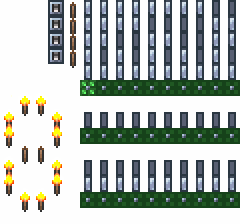
\includegraphics[width=0.3\textwidth]{images/42.png}

\includegraphics[width=0.3\textwidth]{images/43.png}
}
\subfloat[黄线绿线接法]{
\label{i115}

\includegraphics[width=0.3\textwidth]{images/115.png}
}
\subfloat{}
\end{center}
\caption{a连接到02356789,b连接到045689,c连接到01234789,d连接到2345689,e连接到0268,f连接到013456789,g连接到0235689。}
\label{i42:43}
\end{figure}

\section{故障逻辑门}

如果任意的普通逻辑门上有至少一个故障逻辑灯,那么该逻辑门会变为蓝色,称为故障逻辑门。故障逻辑门是一个(不是一类)特殊的逻辑门,无论其下方的普通逻辑门是什么,故障逻辑门的性质是相同的。故障逻辑门与其上最下方的故障逻辑灯之间的普通逻辑灯为有效逻辑灯。当故障逻辑门上有一个故障逻辑灯被激活时,故障逻辑门会在下一个逻辑帧依一定概率激活并把其上所有故障逻辑灯状态设定为“未激活”。该概率等于点亮的有效逻辑灯的数量除以所有有效逻辑灯的数量。请读者对照\autoref{i54:58}仔细揣摩这段话的描述。

\begin{figure}[!ht]
\begin{center}
\subfloat[]{
\label{i54}

\includegraphics{images/54.png}
}
\subfloat[]{
\label{i55}

\includegraphics{images/55.png}
}
\subfloat[]{
\label{i56}

\includegraphics{images/56.png}
}
\subfloat[]{
\label{i57}

\includegraphics{images/57.png}
}
\subfloat[]{
\label{i58}
\includegraphics{images/58.png}
}
\end{center}
\caption{当激活顶端的故障逻辑灯时,故障逻辑门激活的概率分别是:\protect\subref{i54}1/7;\protect\subref{i55}2/7;\protect\subref{i56}6/7;\protect\subref{i57}1/2;\protect\subref{i58}1。}
\label{i54:58}
\end{figure}

只有1个有效逻辑灯的故障逻辑门较特殊。因为该逻辑灯熄灭时对应的概率为0,故障逻辑门一定不激活;当逻辑灯点亮时对应概率为1,故障逻辑门一定激活。使用只有1个有效逻辑灯的故障逻辑门可以进行电路控制。

\subsection{换线器}
在普通逻辑门那里我们已经讲了换线器的做法。简单来说,换线器就是利用某些逻辑门遇输入必输出的特性。在实际应用中换线器的变种非常多。

\begin{figure}[!ht]
\centering
\subfloat[单灯换线器]{\label{fig9}\includegraphics{images/361.png}}
\qquad
\subfloat[双灯换线器]{\label{fig10}\includegraphics{images/362.png}}
\caption{换线器}
\end{figure}

单灯换线器只有一种,就是任何一个普通逻辑门上加一个逻辑灯(\autoref{fig9})。双灯换线器因为有中间的逻辑门隔开,输入和输出可以用同色的线。与门、异或门、故障门都可以做双灯换线器,如\autoref{fig10}所示。

这三种双灯换线器乍看起来又是等价的,然而实际上不是。正因为它们不等价,实际应用中可以利用它们的区别丰富我们的设计思路。

\begin{figure}[!ht]
\centering
\subfloat[与门vs故障门]{\label{fig11}\includegraphics{images/363.png}\quad\includegraphics{images/364.png}}
\qquad
\subfloat[异或门抗干扰]{\label{fig12}\includegraphics{images/365.png}\quad\includegraphics{images/366.png}}
\caption{\protect\subref{fig11}右击开关,红蓝线同时激活,左边火把不响应,右边火把响应;\protect\subref{fig12}无论蓝线如何激活,都不影响换线器工作。}
\end{figure}

首先来看与门和故障门的区别。它们的最上面的逻辑灯激活时,逻辑门都会激活。但是,如果最上面的逻辑灯同时激活两次,与门不会激活,而故障门会激活一次,对应的实验电路如\autoref{fig11}。读者可以自己实验,然后结合普通逻辑门和故障逻辑门的特性描述,思考一下为什么会这样。异或门和故障门也有同样的区别。

再来看与门和异或门的区别。与门不抗干扰,异或门抗干扰。什么意思呢?如\autoref{fig12}所示,有一根与换线器无关的电线想要横穿换线器。对于异或门,只要用图中的方法就可以避免干扰;对于与门,那么无论如何都没法避免横穿的线带来的干扰。读者可自行分析其中原因。可能你会问,有谁会自找麻烦把一根线穿过去?在实际应用中有时不得不这么做,这时异或门就提供了便利。

\subsection{赋值电路}\label{sec14}

泰拉瑞亚中的逻辑电路有个非常大的缺点,就是赋值困难。在数电中,想要给电路赋值0或1,只用连上对应电平的电源即可。然而在泰拉瑞亚中,电线没有电平高低,只有激活,而激活只能改变逻辑灯状态。把一个逻辑灯赋值为0,就需要在这个逻辑灯本来是1的情况下激活一次(或激活奇数次),在逻辑灯本来是0的情况下不激活(或激活偶数次)。如\autoref{i52:53}所示的电路可以做到这一点:当逻辑灯灭时,激活红线会将故障逻辑灯激活,因为逻辑灯灭,逻辑门不激活,逻辑灯保持灭。当逻辑灯亮时,激活红线会将故障逻辑灯激活,因为逻辑灯亮,逻辑门激活蓝线,逻辑灯熄灭。无论如何,激活红线都会使逻辑灯熄灭。

\begin{figure}[!ht]
\begin{center}
\subfloat{
\label{i52}
\includegraphics{images/52.png}
}
\subfloat{
\label{i53}
\includegraphics{images/53.png}
}
\end{center}
\caption{}
\label{i52:53}
\end{figure}

如果将逻辑灯与一个火把同步,就可以做到激活红线使火把熄灭。如果将逻辑灯与火把反向同步,就可以做到激活红线使火把点亮(\autoref{i59:60})。

\begin{figure}[!ht]
\begin{center}
\subfloat{
\label{i59}
\includegraphics{images/59.png}
}
\subfloat{
\label{i60}
\includegraphics{images/60.png}
}
\end{center}
\caption{左边开关使火把点亮(赋值1),右边开关使火把关闭(赋值0)。}
\label{i59:60}
\end{figure}

\begin{example}[D触发器]\label{sec15}

\begin{figure}[!ht]
\begin{center}
\subfloat{
\label{i237}
\includegraphics{images/237.png}
}
\qquad
\subfloat{
\label{i238}
\includegraphics{images/238.png}
}
\end{center}
\caption{左边的开关改变A火把的状态,右边的开关将A火把状态更新到B火把。}
\label{i237:238}
\end{figure}

D触发器是数电的术语,其功能非常简单,就是存储并发送状态。见\autoref{i237:238},左边的开关可以随意控制左边的火把,而右边的开关会使得右边的火把和左边的火把状态同步。换言之,D触发器存储了左边火把的值,而右边的开关命令D触发器将它存储的值发出。

回顾\nameref{sec14},它可以把火把的值设定为一个常数,而该常数可以通过故障逻辑门上的有效逻辑灯来调节。而在\autoref{i237:238}中,我们让左边的火把来调节故障逻辑门上的有效逻辑灯,当左边火把为1时,故障逻辑门的作用是赋值1;当左边火把为0时,故障逻辑门的作用是赋值0。这样一来,这个故障逻辑门的功能实际上是把右边火把的值赋值为左边火把的值。
\end{example}

\subsection{递次电路}\label{sec35}

递次电路是使用频率非常高的电路。传统的递次电路如\autoref{i72:73}所示。当激活绿线时,一排故障逻辑灯被激活。但是由于只有第一个有效逻辑灯是亮的,只有第一个故障逻辑门激活,从而第一个有效逻辑灯熄灭,第二个有效逻辑灯被点亮。当再次激活绿线时,同理,第二个故障逻辑门激活,第二个有效逻辑灯熄灭,第三个有效逻辑灯点亮。依此进行,当反复激活绿线时,六个故障逻辑门依次激活并循环。将每个故障逻辑门接出一个电路,就可以实现六个电路依次运行并循环。

\begin{figure}[!ht]
\begin{center}
\subfloat{
\label{i72}
\includegraphics{images/72.png}
}
\subfloat{
\label{i73}
\includegraphics{images/73.png}
}
\end{center}
\caption{}
\label{i72:73}
\end{figure}

实际应用中的递次电路非常灵活。不仅故障逻辑门的数量可以随意变化,有效逻辑灯的亮灭、接线方式都可以视实际需求变化。递次电路的常见变种见\autoref{sec2}。使用递次电路时不要死板,要善于针对需求设计最合理的电路。

递次电路的使用非常广泛。它可以与十进制数显结合做成\url{https://www.bilibili.com/video/av22894193}中的十进制计数器,也可以做出\url{https://www.bilibili.com/video/av21009075}中的霓虹灯效果,还可以做出\url{https://www.bilibili.com/video/av6393957}中的回血回蓝大阵,等等等等等等。

递次电路的另一个典型用途就是降频。我们知道,传送带驱动的频率是60Hz。现在我们需要20Hz的驱动,只需要利用循环长度为3的递次电路(\autoref{i90:91})。

\begin{figure}[!ht]
\begin{center}
\subfloat{
\label{i90}
\includegraphics{images/90.png}
}
\subfloat{
\label{i91}
\includegraphics{images/91.png}
}
\end{center}
\caption{将黄线接出即得到20Hz的驱动,因为绿线每激活3次,黄线都激活1次。}
\label{i90:91}
\end{figure}

在一些时候,比如上面提到的十进制计数器中,我们需要“清零”操作,即将递次电路复位到初始状态。使用\nameref{sec14}很容易实现这一点(\autoref{i86:87})。但是这里想说明的是,对赋值对象的理解需要非常灵活。

\begin{figure}[!ht]
\begin{center}
\subfloat{
\label{i86}
\includegraphics{images/86.png}
}
\subfloat{
\label{i87}
\includegraphics{images/87.png}
}
\end{center}
\caption{上面的开关用来正常激活递次电路,下面的开关用来复位。除了横穿所有故障逻辑灯的绿线和黄线外,红线和蓝线用来进行递次电路中的循环并将上面有效逻辑灯的状态同步到下面,绿线和黄线用来赋值。多加一排故障逻辑灯是为了将颜色冲突的线分开。}
\label{i86:87}
\end{figure}

是不是只有逻辑灯才有状态?在递次电路中,电线也可以有状态。如果我们把每根电线接到一个火把,就可以把火把的状态看作电线的状态。那么与其对逻辑灯赋值,不如直接对电线赋值,电路如\autoref{i88:89}所示。对电线进行赋值的前提是电线状态可以决定逻辑灯的状态。

\begin{figure}[!ht]
\begin{center}
\subfloat{
\label{i88}
\includegraphics{images/88.png}
}
\subfloat{
\label{i89}
\includegraphics{images/89.png}
}
\end{center}
\caption{上面的开关用来正常激活递次电路,下面的开关用来复位。}
\label{i88:89}
\end{figure}

将\autoref{i88:89}中下面一排复位电路穿插到上面递次电路的缝隙里,可以得到占用空间更小的版本(\autoref{i106:107})。

\begin{figure}[!ht]
\begin{center}
\subfloat{
\label{i106}
\includegraphics{images/106.png}
}
\subfloat{
\label{i107}
\includegraphics{images/107.png}
}
\end{center}
\caption{上面的开关用来正常激活递次电路,下面的开关用来复位。}
\label{i106:107}
\end{figure}

另外,偶尔我们可能需要用到双向递次电路,它的各种做法见\autoref{sec3}。

\subsection{降频电路}\label{sec2:1}

我们已经讲过了如何利用递次电路降频。例如\autoref{i92:97}\subref{i92:93}中,绿线激活奇数次时红线激活,偶数次时蓝线激活。事实上降频一半有更简单的方式。在\autoref{i92:97}\subref{i94:95}中,激活绿线会激活故障逻辑灯并同时点亮有效逻辑灯,此时故障逻辑门会激活,红线激活;再次激活绿线会激活故障逻辑灯并同时熄灭有效逻辑灯,此时故障逻辑门不激活。\autoref{i92:97}\subref{i94:95}也可以做到在绿线激活奇数次时红线激活,\autoref{i92:97}\subref{i96:97}也可以做到在绿线激活偶数次时蓝线激活。一般说的降频电路就指这种使用一个故障逻辑门,把频率降低一半的电路。一般不要求精确频率时,使用降频电路比递次电路更节省空间。

\begin{figure}[!ht]
\begin{center}
\subfloat[]{
\label{i92:93}
\includegraphics{images/92.png}
\includegraphics{images/93.png}
}
\qquad
\subfloat[]{
\label{i94:95}
\includegraphics{images/94.png}
\includegraphics{images/95.png}
}
\qquad
\subfloat[]{
\label{i96:97}
\includegraphics{images/96.png}
\includegraphics{images/97.png}
}
\end{center}
\caption{}
\label{i92:97}
\end{figure}

\subsection{十进制计数器}

在这一小节中我们将使用之前学过的模块来做一个四位带数显的十进制计数器。

计数器计数的对象是驱动或某个特定的信号源。信号源每激活一次,计数器的数字加1。因为是十进制,所以满十进一,这提示我们使用循环为10的递次电路作为计数模块。因为计数器要有清零功能,所以递次电路要带上复位电路。根据数字的书写习惯,右边低位,左边高位,所以采用反向的递次电路并且将逻辑门稍微错位使接线更顺。将低位的递次电路最后一个逻辑门的输出接上高一位递次电路的输入即可完成进位功能(\autoref{i108:109}),然后将最低位的递次电路输入接上驱动的输出即可以实现计数功能。

\begin{figure}[!ht]
\begin{center}
\subfloat{
\label{i108}
\includegraphics[width=0.9\textwidth]{images/108.png}
}
\\
\subfloat{
\label{i109}
\includegraphics[width=0.9\textwidth]{images/109.png}
}
\end{center}
\caption{绿线计数,黄线复位。最右边是个位,最左边是千位。}
\label{i108:109}
\end{figure}

对递次电路熟悉的人通过递次电路上的逻辑灯已经可以读出数字:递次电路上最右边的有效逻辑灯亮代表这一位是0,最左边的有效逻辑灯亮代表这一位是9。但是既然要面向不懂电路的用户,就需要把数字可视化,即加上数显。我们在之前已经做过一个十进制的数显,如果将那个数显的显示部分照搬过来,很容易发现显示的不对,这是因为两个数显的输入不同。之前做的数显,数字改变时显示器收到两个信号:第一个信号将之前的数字熄灭,第二个信号将新的数字点亮。而我们的递次电路的输出只是之前的数字。因为计数器中之前的数字可以唯一确定新的数字,所以我们可以直接让递次电路发出的信号激活从旧数字变成新数字需要激活的火把。另外,由于显示器是多个数字排列在一起,为了避免接线困难,应当先把数字上的线确定好,再往递次电路上接。如果选用\autoref{i110:112}\subref{i110}所示的火把排布,由于数字间只空了一格,之前用过的七段线接法就不能用了。所以我们采用的另一种七段线接法\autoref{i110:112}\subref{i112},注意某些线有重叠。利用\autoref{jishuqi}就可以完成接线(\autoref{i113:114})。注意到这里使用了故障逻辑门做换线器。

\begin{figure}[!ht]
\begin{center}
\subfloat[]{
\label{i110}
\includegraphics[width=0.45\textwidth]{images/110.png}
}
\subfloat[]{
\label{i112}
\includegraphics[width=0.45\textwidth]{images/112.png}
}
\end{center}
\caption{}
\label{i110:112}
\end{figure}

\begin{table}[!ht]
\centering
\begin{tabular}{c|c|c|c|c|c|c|c|c|c|c}
数字变化&0$\to$1&1$\to$2&2$\to$3&3$\to$4&4$\to$5&5$\to$6&6$\to$7&7$\to$8&8$\to$9&9$\to$0\\
\hline
激活部分&ad&abdeg&bcfg&abcd&acdf&bc&de&def&bc&bcef
\end{tabular}
\caption{}
\label{jishuqi}
\end{table}

\begin{figure}[!ht]
\begin{center}
\subfloat{
\label{i113}
\includegraphics[width=0.9\textwidth]{images/113.png}
}
\\
\subfloat{
\label{i114}
\includegraphics[width=0.9\textwidth]{images/114.png}
}
\end{center}
\caption{}
\label{i113:114}
\end{figure}

\subsection{降频技术}\label{sec18}
灵活使用递次电路和降频电路可以将已有的驱动时长增加为任意整数倍(\autoref{i223:228})。

\begin{figure}[!ht]
\begin{center}
\subfloat[]{
\label{i223:224}
\includegraphics{images/223.png}
\includegraphics{images/224.png}
}
\qquad
\subfloat[]{
\label{i225:226}
\includegraphics{images/225.png}
\includegraphics{images/226.png}
}
\qquad
\subfloat[]{
\label{i227:228}
\includegraphics{images/227.png}
\includegraphics{images/228.png}
}
\end{center}
\caption{\protect\subref{i223:224}两个降频电路连接,红线每激活4次火把响应一次;\protect\subref{i225:226}两个递次电路连接,红线每激活9次火把响应一次;\protect\subref{i227:228}降频电路与递次电路连接,红线每激活6次火把响应一次。}
\label{i223:228}
\end{figure}

使用上面的方法,当需要获得较大的质数倍(例如23倍)时间时使用递次电路体积过大,此时可以利用故障逻辑门的控制功能灵活地将多个降频的驱动结合(\autoref{i231:232})。这实质上是一个\hyperref[sec5]{多级递次}。

\begin{figure}[!ht]
\begin{center}
\subfloat{
\label{i231}
\includegraphics{images/231.png}
}
\qquad
\subfloat{
\label{i232}
\includegraphics{images/232.png}
}
\end{center}
\caption{开关每激活23次火把响应一次。上面的右边两个故障逻辑门用来控制,左边的输出接到计数为20的模块(5-递次电路与两个降频电路连接),右边的输出接到3-递次电路。开关激活时,起初左边输出,右边不输出,左边计数。当左边计数到20时上面的绿线激活,改变控制用的有效逻辑灯,改为右边输出,左边不输出,右边计数。当右边计数到3时激活火把并将控制用的有效逻辑灯改回。}
\label{i231:232}
\end{figure}

\subsection{骰子}

在前面的例子中,我们仅使用了有一个有效逻辑灯的故障逻辑门的控制功能。在这个例子中我们来使用故障逻辑门的概率功能。我们的目标是做一个电路,该电路有一个开关和六个火把。当激活开关时,六个输出有且仅有一个点亮,且每个火把点亮的概率都为1/6。

电路如\autoref{i98:99}所示。激活顶端黄线即可运行。下面很明显是递次电路,我们先分析上面部分,看看绿线会激活多少次。

\begin{figure}[!ht]
\begin{center}
\subfloat{
\label{i98}
\includegraphics{images/98.png}
}
\subfloat{
\label{i99}
\includegraphics{images/99.png}
}
\end{center}
\caption{}
\label{i98:99}
\end{figure}

当顶端黄线激活时,第一个故障逻辑门有5/6的概率激活。只有第一个故障逻辑门激活的前提下,后面的故障逻辑门才有可能激活,也就是说,有1-5/6=1/6的概率一次也不激活。在第一个故障逻辑门激活的前提下,第二个故障逻辑门有4/5的概率激活。只有第二个故障逻辑门激活的前提下,后面的故障逻辑门才有可能激活,也就是说,有5/6*(1-4/5)=1/6的概率仅第一个故障逻辑门激活,此时绿线激活一次。依此类推,可以得到绿线有5/6*4/5*(1-3/4)=1/6的概率激活两次,有5/6*4/5*3/4*(1-2/3)=1/6的概率激活三次,有5/6*4/5*3/4*2/3*(1-1/2)=1/6的概率激活四次,有5/6*4/5*3/4*2/3*1/2=1/6的概率激活五次。也就是说,顶端黄线激活时,绿线等可能地激活0\~{}5次。

绿线等可能地激活0\~{}5次,经过下面的递次电路,就会导致点亮的火把等可能地循环右移0\~{}5个。无论激活顶端黄线之前哪个火把是亮的,这都意味着六个火把有等可能的概率点亮。

\begin{problemset}[思考题]
\item 为什么只能由玩家激活的压力板会选用灰/棕/蓝/丛林蜥蜴这四种颜色?
\item 解释为什么如\autoref{i11:12}所示装置会在世界开启瞬间激活广播盒。该装置里的故障逻辑门有什么作用?
\begin{figure}[!ht]
\begin{center}
\subfloat{
\label{i11}
\includegraphics[width=0.4\textwidth]{images/11.png}
}
\subfloat{
\label{i12}
\includegraphics[width=0.4\textwidth]{images/12.png}
}
\end{center}
\caption{}
\label{i11:12}
\end{figure}
\item 制作一个装置,在每天入昼时显示讯息“日食正在发生...”,入夜时显示“血月正在升起...”。
\item 找出\url{https://www.bilibili.com/video/av5271577}中的延时装置。
\item 做一个显示当前月相的显示器,显示效果如\autoref{i61:68}。
\begin{figure}[!ht]
\begin{center}
\subfloat[满月]{
\label{i61}
\includegraphics[width=0.11\textwidth]{images/61.png}
}
\subfloat[亏凸月]{
\label{i62}
\includegraphics[width=0.11\textwidth]{images/62.png}
}
\subfloat[下弦月]{
\label{i63}
\includegraphics[width=0.11\textwidth]{images/63.png}
}
\subfloat[残月]{
\label{i64}
\includegraphics[width=0.11\textwidth]{images/64.png}
}
\subfloat[新月]{
\label{i65}
\includegraphics[width=0.11\textwidth]{images/65.png}
}
\subfloat[峨眉月]{
\label{i66}
\includegraphics[width=0.11\textwidth]{images/66.png}
}
\subfloat[上弦月]{
\label{i67}
\includegraphics[width=0.11\textwidth]{images/67.png}
}
\subfloat[盈凸月]{
\label{i68}
\includegraphics[width=0.11\textwidth]{images/68.png}
}
\end{center}
\caption{}
\label{i61:68}
\end{figure}
\item 实现\url{https://www.bilibili.com/video/av5271577} 2分57秒处神庙尖刺的效果。
\item 设计如\autoref{i69:70}所示的二进制数显。
\begin{figure}[!ht]
\begin{center}
\subfloat[0]{
\label{i69}
\includegraphics{images/69.png}
}
\qquad
\subfloat[1]{
\label{i70}
\includegraphics{images/70.png}
}
\end{center}
\caption{}
\label{i69:70}
\end{figure}
\item 补全十进制数显\autoref{i71}的接线。
\begin{figure}[!ht]
\centering
\includegraphics{images/71.png}
\caption{}
\label{i71}
\end{figure}
\item 为什么十进制带数显的计数器一般不会多于四位?
\item 利用降频电路和二进制数显制作一个多位的二进制计数器。
\item 做一个可以显示点数的骰子,六个点数效果如\autoref{i100:105}。
\begin{figure}[!ht]
\begin{center}
\subfloat[1]{
\label{i100}
\includegraphics[width=0.15\textwidth]{images/100.png}
}
\subfloat[2]{
\label{i101}
\includegraphics[width=0.15\textwidth]{images/101.png}
}
\subfloat[3]{
\label{i102}
\includegraphics[width=0.15\textwidth]{images/102.png}
}
\subfloat[4]{
\label{i103}
\includegraphics[width=0.15\textwidth]{images/103.png}
}
\subfloat[5]{
\label{i104}
\includegraphics[width=0.15\textwidth]{images/104.png}
}
\subfloat[6]{
\label{i105}
\includegraphics[width=0.15\textwidth]{images/105.png}
}
\end{center}
\caption{}
\label{i100:105}
\end{figure}
\end{problemset}